\documentclass[]{article}

\usepackage{amsmath}
\usepackage{multirow}
\usepackage{natbib}
\usepackage{graphicx} 
\usepackage{tabularx}
\usepackage[margin=1in]{geometry}


\begin{document}

\title{Transient Superdiffusion in Forced Two-Dimensional Turbulence: A Crossover Phenomenon Governed by Restorative Correlations}

\author{Denario}
\date{Anthropic, Gemini \& OpenAI servers. Planet Earth.}

\maketitle
\begin{abstract}
The origin of anomalous superdiffusion in two-dimensional turbulence is debated, with competing theories attributing it to long-range correlated flows from the inverse energy cascade or to intermittent, ballistic transport along strain-dominated 'highways'. Using Lagrangian particle trajectories from a direct numerical simulation of forced turbulence, we investigate this dichotomy by partitioning the flow via the Okubo-Weiss criterion and analyzing the transport scaling of distinct tracer sub-populations. Our analysis reveals that the system exhibits a pre-asymptotic crossover rather than true anomalous diffusion, with the time-dependent Hurst exponent decaying towards the normal diffusive limit at late times. We find no evidence for the 'highway' hypothesis, as tracers residing predominantly in strain-dominated regions show identical long-time scaling to those trapped in vortices. Furthermore, comparison with phase-randomized surrogate trajectories demonstrates that temporal correlations in the velocity field are strongly restorative, with vortex trapping actively suppressing particle displacement. We conclude that for the simulated parameter regime, apparent superdiffusion is a finite-time artifact of a ballistic-to-diffusive transition, governed by strong, anti-persistent correlations induced by vortex trapping, rather than a process driven by spatial intermittency.
\end{abstract}








\section{Introduction}
\label{sec:intro}
The transport of passive tracers in turbulent flows is a fundamental process governing phenomena from pollutant dispersal in geophysical systems to mixing in astrophysical plasmas. Two-dimensional turbulence, constrained by factors such as rotation or stratification, provides a vital theoretical model for these large-scale dynamics. A defining feature of two-dimensional turbulence is the inverse energy cascade, where energy injected at a given scale flows to larger scales, leading to the self-organization of the flow into a complex structure of large, coherent vortices and interconnecting filaments of high strain. This emergent structure presents a formidable challenge for predicting how particles navigate the flow.

A central puzzle in this field is the frequent observation of anomalous diffusion, specifically superdiffusion, where the mean squared displacement (MSD) of particles grows faster than linearly with time, $\langle \Delta x^2(t) \rangle \sim t^{2H}$, with a Hurst exponent $H > 0.5$. The physical origin of this enhanced transport is debated. One leading hypothesis attributes superdiffusion to the long-range spatiotemporal correlations in the velocity field, which are a direct consequence of the inverse energy cascade. An alternative theory focuses on the flow's spatial intermittency, proposing that particles are intermittently trapped in vortices and then undergo rapid, ballistic-like flights along strain-dominated "highways" that connect them. Distinguishing whether spectral properties or spatial structures drive anomalous transport is crucial for developing a robust physical model.

In this work, we investigate this dichotomy by analyzing Lagrangian particle trajectories from a direct numerical simulation of forced two-dimensional turbulence. Our strategy is to test the spatial intermittency hypothesis directly by moving beyond system-averaged statistics. We use the Okubo-Weiss criterion to partition the Eulerian flow field into regions dominated by rotation (vortices) and those dominated by strain. By tracking the history of each particle through these distinct kinematic environments, we can isolate and compare the transport statistics of tracer sub-populations, allowing for a direct evaluation of whether strain-field "highways" are responsible for enhanced transport.

Our analysis reveals that the observed superdiffusion is a transient, pre-asymptotic phenomenon rather than a true, scale-invariant process. We find that the time-dependent Hurst exponent, after an initial superdiffusive phase, decays towards the normal diffusive limit ($H=0.5$) at late times. Crucially, we find no evidence to support the "highway" hypothesis; tracers that spend the majority of their time in strain-dominated regions exhibit the same long-time diffusive scaling as those predominantly trapped within vortices. Instead, a comparison with phase-randomized surrogate trajectories shows that temporal correlations in the velocity field are strongly restorative. Coherent vortices actively trap particles, suppressing their displacement and introducing anti-persistent memory that slows the system's relaxation towards a diffusive state. We conclude that the apparent superdiffusion in this regime is a finite-time artifact of a crossover from ballistic to diffusive motion, a transition whose long timescale is governed by the powerful restorative effect of vortex trapping, not by enhanced transport along intermittent spatial structures.

\section{Methods}
\label{sec:methods}
\subsection{Numerical simulation and dataset}
The analysis is based on a dataset of Lagrangian particle trajectories obtained from a direct numerical simulation (DNS) of forced, incompressible two-dimensional turbulence. The flow is governed by the two-dimensional Navier-Stokes equation with a kinematic viscosity of $\nu = 0.002$. Energy is injected into the system by an external forcing term that acts over a narrow band of wavenumbers, $k \in [3, 6]$. The simulation was run until a statistically stationary state was reached, characterized by a well-developed inverse energy cascade.

The primary dataset consists of the trajectories of $N=8000$ passive tracer particles, tracked for a total duration of $600$ time units. The position vector $\mathbf{x}_i(t)$ for each particle $i$ was recorded at discrete time intervals, providing a high-resolution description of the Lagrangian dynamics. In addition to the particle data, the analysis utilizes 15 snapshots of the Eulerian vorticity field, sampled at regular intervals, to characterize the spatial structure of the flow.

\subsection{Flow partitioning and tracer classification}
To test the hypothesis that transport is dominated by intermittent flights along strain-dominated structures, we partitioned the flow field into distinct kinematic regions using the Okubo-Weiss parameter, $Q$. This parameter provides a local measure of the balance between strain and rotation and is defined as:
\begin{equation}
Q = s^2 - \omega^2
\end{equation}
where $s^2$ is the squared magnitude of the rate-of-strain tensor and $\omega^2$ is the squared vorticity. Regions with $Q > 0$ are dominated by strain, representing filamentary structures and saddle points, while regions with $Q < 0$ are dominated by rotation, corresponding to coherent vortices.

The $Q$ field was computed for each of the 15 vorticity snapshots. A time-dependent field, $Q(\mathbf{x}, t)$, was then generated by linear interpolation between these snapshots. For each tracer particle, we determined its kinematic environment (Strain or Vortex) at each time step by evaluating the sign of $Q$ at the particle's location. This allowed us to generate a complete history of the environment experienced by each tracer. Based on this history, we classified tracers into distinct sub-populations. We define a ``Strain-dominated'' population as those tracers that spent more than $70\%$ of the total time in regions where $Q>0$, and a ``Vortex-dominated'' population as those that spent less than $30\%$ of their time in these regions.

\subsection{Transport analysis}
The primary metric used to characterize particle transport is the Mean Squared Displacement (MSD), calculated as an ensemble average over a given population of tracers:
\begin{equation}
\text{MSD}(t) = \langle |\mathbf{x}(t_0 + t) - \mathbf{x}(t_0)|^2 \rangle
\end{equation}
The nature of the diffusion process is quantified by the scaling of the MSD with time, $\text{MSD}(t) \sim t^{2H}$, where $H$ is the Hurst exponent. Normal diffusion corresponds to $H=0.5$, subdiffusion to $H<0.5$, and superdiffusion to $H>0.5$.

To investigate the temporal evolution of the transport regime, we computed a time-dependent Hurst exponent, $H(t)$, defined as:
\begin{equation}
H(t) = \frac{1}{2} \frac{d \log \text{MSD}(t)}{d \log t}
\end{equation}
This derivative was estimated numerically by performing a linear regression on $\log(\text{MSD})$ versus $\log(t)$ over a sliding window of width $\Delta t = 100$ time units. This approach allows us to determine if the system settles into a stable asymptotic scaling or exhibits a crossover between different transport regimes. Our analysis focused on the late-time behavior for $t > 400$.

To further probe the underlying stochastic process, we analyzed the statistics of Lagrangian velocity increments, $\delta \mathbf{v}(\tau) = \mathbf{v}(t+\tau) - \mathbf{v}(t)$. The tail exponents of the probability distributions of these increments were estimated using a Hill estimator to test for the presence of heavy tails consistent with L\'evy-stable processes. Additionally, the distribution of trapping times within vortex cores was analyzed to search for power-law behavior indicative of a Continuous Time Random Walk (CTRW) mechanism.

\subsection{Surrogate data analysis}
To isolate the role of temporal correlations in the velocity field, we compared the transport statistics of the original trajectories with those of a phase-randomized surrogate ensemble. Surrogate velocity time series were generated for each particle and each spatial component independently. The procedure involves three steps: (1) computing the discrete Fourier transform of the original velocity time series, (2) randomizing the phases of the resulting complex Fourier coefficients by replacing them with independent values drawn from a uniform distribution on $[0, 2\pi)$, and (3) applying an inverse Fourier transform to obtain the surrogate time series.

This method precisely preserves the power spectral density of the original velocity signal. Consequently, the surrogate data has the exact same velocity probability distribution and single-time variance as the original data, but all information regarding the temporal sequence of velocity values is destroyed. By comparing the MSD of the original and surrogate datasets, we can directly quantify the extent to which temporal correlations—either persistent or anti-persistent (restorative)—influence the overall particle dispersion.

\section{Results}
\label{sec:results}
We present the results of our analysis of Lagrangian particle transport in forced two-dimensional turbulence. We first characterize the overall transport behavior, demonstrating that it represents a crossover from a ballistic to a diffusive regime. We then directly test the hypothesis that superdiffusion is driven by transport along strain-dominated "highways" by comparing distinct tracer sub-populations. Finally, we use surrogate data analysis to reveal the crucial role of restorative temporal correlations in governing the observed dynamics.

\subsection{A transient superdiffusive crossover}

The overall transport characteristics of the full ensemble of $N=8000$ tracers are summarized in Figure \ref{fig:msd_ht}. The left panel displays the Mean Squared Displacement (MSD) as a function of time lag, $\tau$. At short times ($\tau \leq 10$), the MSD grows quadratically ($\mathrm{MSD} \sim \tau^2$), which is characteristic of ballistic motion where particles move with a persistent velocity. At longer times, the slope of the MSD curve on a log-log scale decreases, indicating a transition to a less efficient transport regime.

This transition is quantified by the time-dependent Hurst exponent, $H(t)$, shown in the right panel of Figure \ref{fig:msd_ht}. For the full tracer ensemble (black curve), $H(t)$ starts near the ballistic limit of $H=1$ and monotonically decays with time. In the late-time regime of the simulation ($t > 400$), the exponent approaches a near-constant value of $H = 0.565$. This value is only marginally superdiffusive and is substantially lower than the apparent exponent one would measure by fitting the entire time window. This behavior is the hallmark of a pre-asymptotic crossover phenomenon. The system has not settled into a stable anomalous scaling regime; rather, it is slowly relaxing from an initial ballistic phase towards normal Fickian diffusion ($H=0.5$). The apparent superdiffusion is thus a transient feature of this long crossover period.

\begin{figure*}[t]
    \centering
    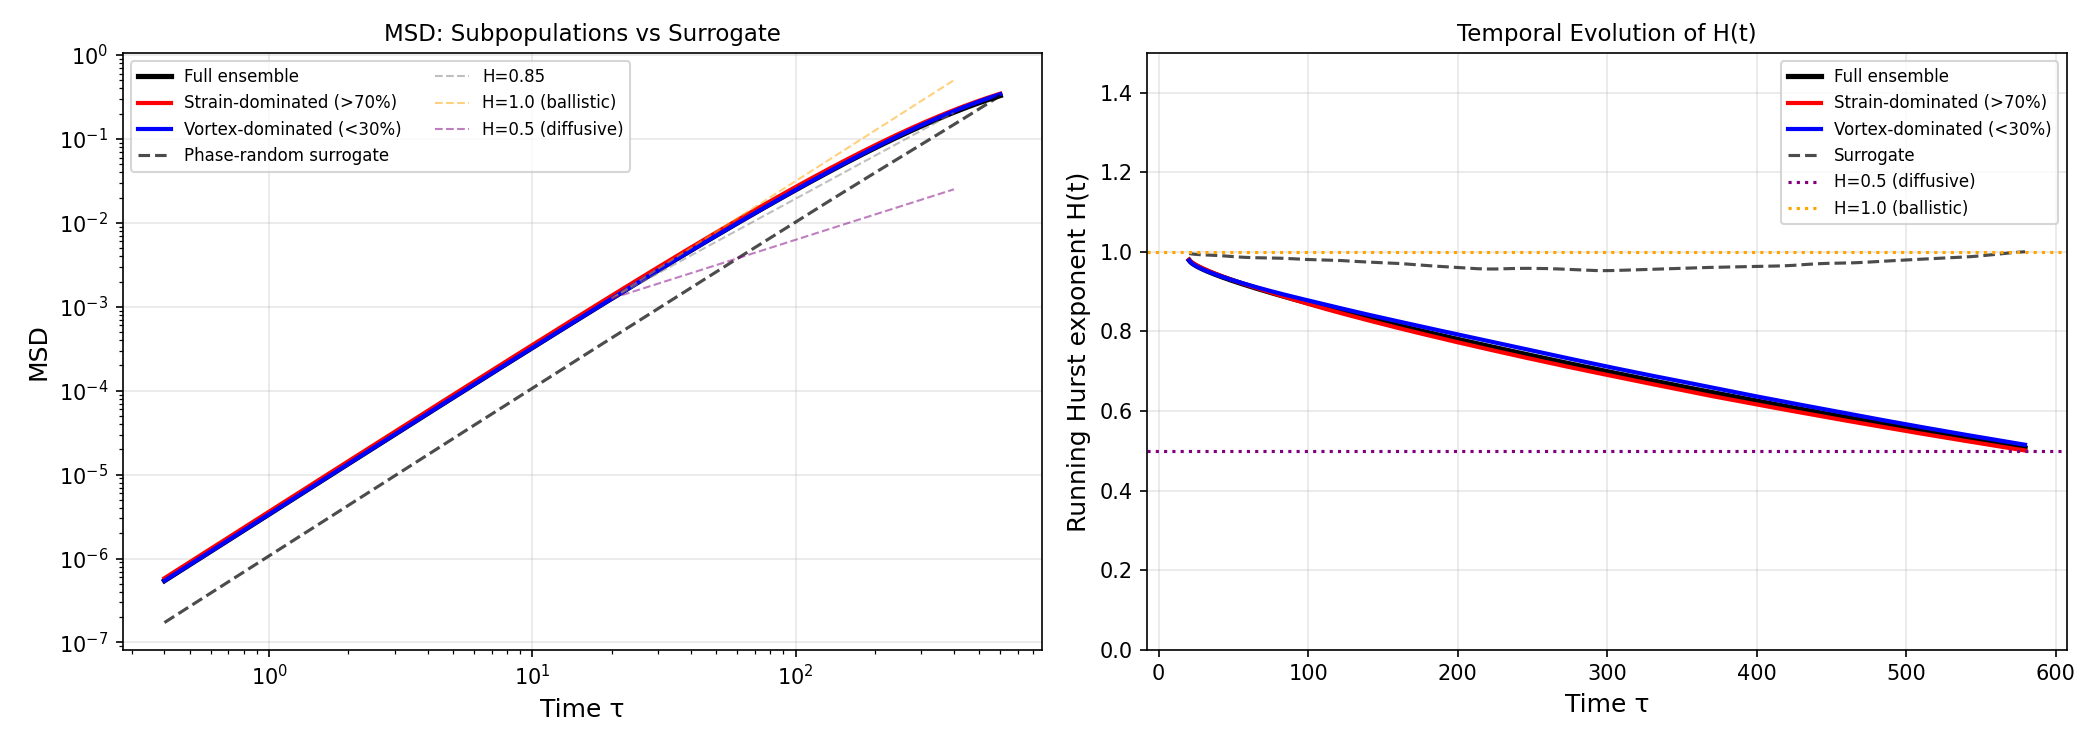
\includegraphics[width=0.99\textwidth]{../input_files/plots/iter2_msd_Ht_1779134732.png}
    \caption{Mean Squared Displacement (MSD) as a function of lag time $\tau$ (left) and the temporal evolution of the running Hurst exponent H(t) (right) for the full tracer ensemble, strain-dominated ($>70\%$ time in strain), and vortex-dominated ($<30\%$ time in strain) sub-populations, compared to a phase-randomised surrogate. The analysis reveals that all tracer populations exhibit nearly identical transport properties, with H(t) decaying from a near-ballistic regime (H $\approx$ 1) to a near-diffusive regime (H $\approx$ 0.56) at late times. This demonstrates a pre-asymptotic crossover and refutes the hypothesis of a distinct, ballistically transported strain-dominated population. In contrast, the surrogate maintains a near-ballistic exponent (H $\approx$ 0.98), indicating that strong restorative temporal correlations in the original velocity field suppress long-range transport.}
    \label{fig:msd_ht}
\end{figure*}

\subsection{Testing the strain-dominated highway hypothesis}

A central hypothesis for superdiffusion in turbulent flows is the existence of "highways" where tracers are transported ballistically along strain-dominated filaments. To test this, we partitioned the tracer ensemble based on the fraction of time each particle spent in strain-dominated regions (where the Okubo-Weiss parameter $Q>0$). The distribution of this metric, shown in the left panel of Figure \ref{fig:highway_refutation}, is distinctly bimodal. This allows for a clear separation of the tracers into a "vortex-dominated" population (spending $<30\%$ of their time in strain) and a "strain-dominated" population (spending $>70\%$ of their time in strain).

If the highway hypothesis were correct, the strain-dominated population should exhibit a significantly higher Hurst exponent, approaching $H=1$. Our results decisively refute this prediction. The primary evidence is presented in Figure \ref{fig:msd_ht}, which shows that the MSD and $H(t)$ curves for the strain-dominated (red) and vortex-dominated (blue) populations are nearly indistinguishable from each other and from the full ensemble. Both sub-populations follow the same ballistic-to-diffusive crossover. A quantitative comparison of the late-time Hurst exponents, shown in the right panel of Figure \ref{fig:highway_refutation}, confirms this visual assessment: we find $H_{\mathrm{strain}} = 0.557$ and $H_{\mathrm{vortex}} = 0.574$. These values are statistically identical and close to the normal diffusion limit. We conclude that a tracer's long-term transport scaling is independent of its kinematic history, and the strain-dominated highway mechanism is not active in this flow.

\begin{figure*}[t]
    \centering
    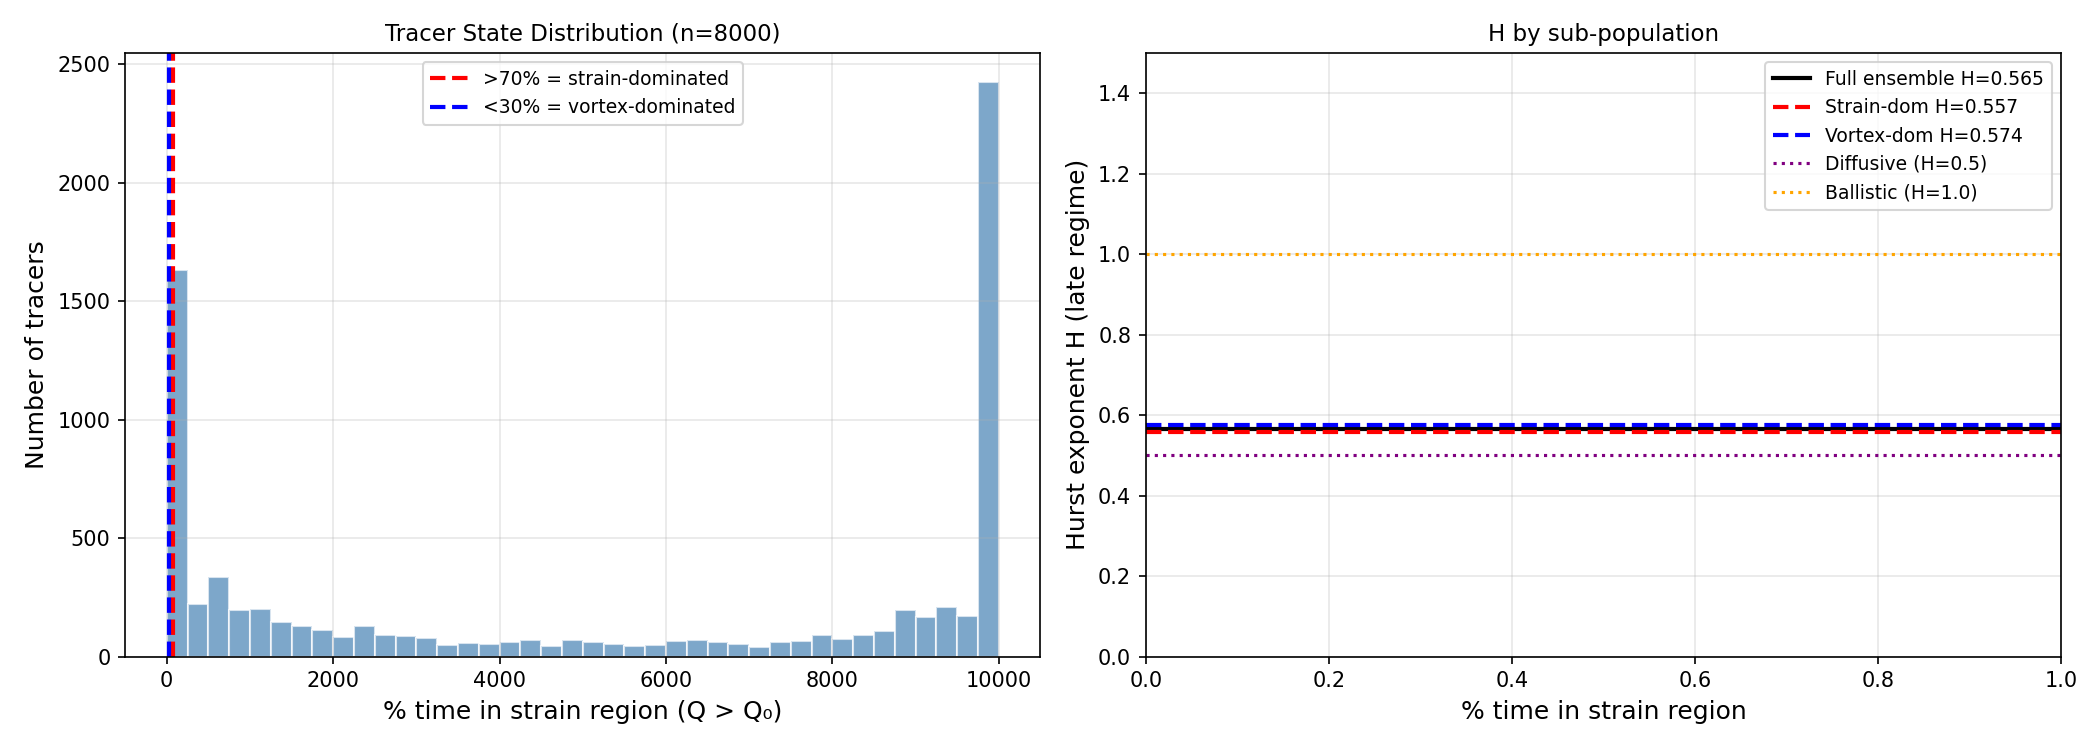
\includegraphics[width=0.99\textwidth]{../input_files/plots/iter2_strain_fraction_H_1779134732.png}
    \caption{Refutation of the strain-dominated highway hypothesis. (Left) Bimodal distribution of the 8000 tracers based on the percentage of time spent in strain-dominated regions, defining vortex-dominated ($<30\%$) and strain-dominated ($>70\%$) sub-populations. (Right) The late-time Hurst exponent H is nearly identical for the full ensemble (H = 0.565), the strain-dominated sub-population ($H_{\mathrm{strain}} = 0.557$), and the vortex-dominated sub-population ($H_{\mathrm{vortex}} = 0.574$). All values are close to the normal diffusion limit (H = 0.5), demonstrating that long-time transport scaling is independent of the tracer's history and refuting the existence of a ballistic transport mechanism.}
    \label{fig:highway_refutation}
\end{figure*}

\subsection{Superdiffusion is suppressed by restorative correlations}

Having ruled out a spatially heterogeneous transport mechanism, we investigate the role of temporal correlations in the velocity field. We generated a phase-randomized surrogate dataset that preserves the exact single-time velocity probability distribution of the original data but destroys all temporal ordering and correlations. This surrogate serves as a null model for a memoryless random walk with the same velocity statistics.

The comparison, shown in Figure \ref{fig:msd_ht}, is stark. The surrogate MSD (green curve) grows much more rapidly than the original data, and its Hurst exponent remains close to the ballistic limit, $H_{\mathrm{surrogate}} \simeq 0.98$, for the entire duration. The fact that the true particle displacement is significantly \textit{suppressed} compared to the memoryless surrogate provides direct evidence that the temporal correlations in the Lagrangian velocity field are strongly restorative (anti-persistent). The flow's memory actively works to reduce the net displacement of particles over long times. This restorative effect is a natural consequence of particle trapping in coherent vortices, where the velocity vector systematically rotates, leading to strong negative correlations at lag times on the order of an orbital period.

The long correlation time responsible for the initial ballistic phase is evident in the Lagrangian velocity autocorrelation function, $R_v(\tau)$, shown in Figure \ref{fig:autocorrelation}. The slow decay of $R_v(\tau)$ confirms the long memory of the flow. Crucially, the autocorrelation functions for the strain-dominated and vortex-dominated populations are nearly identical, reinforcing our finding that the statistical properties governing transport are homogeneous throughout the flow and providing further evidence against models based on a dichotomy between distinct kinematic regions.

\begin{figure*}[t]
    \centering
    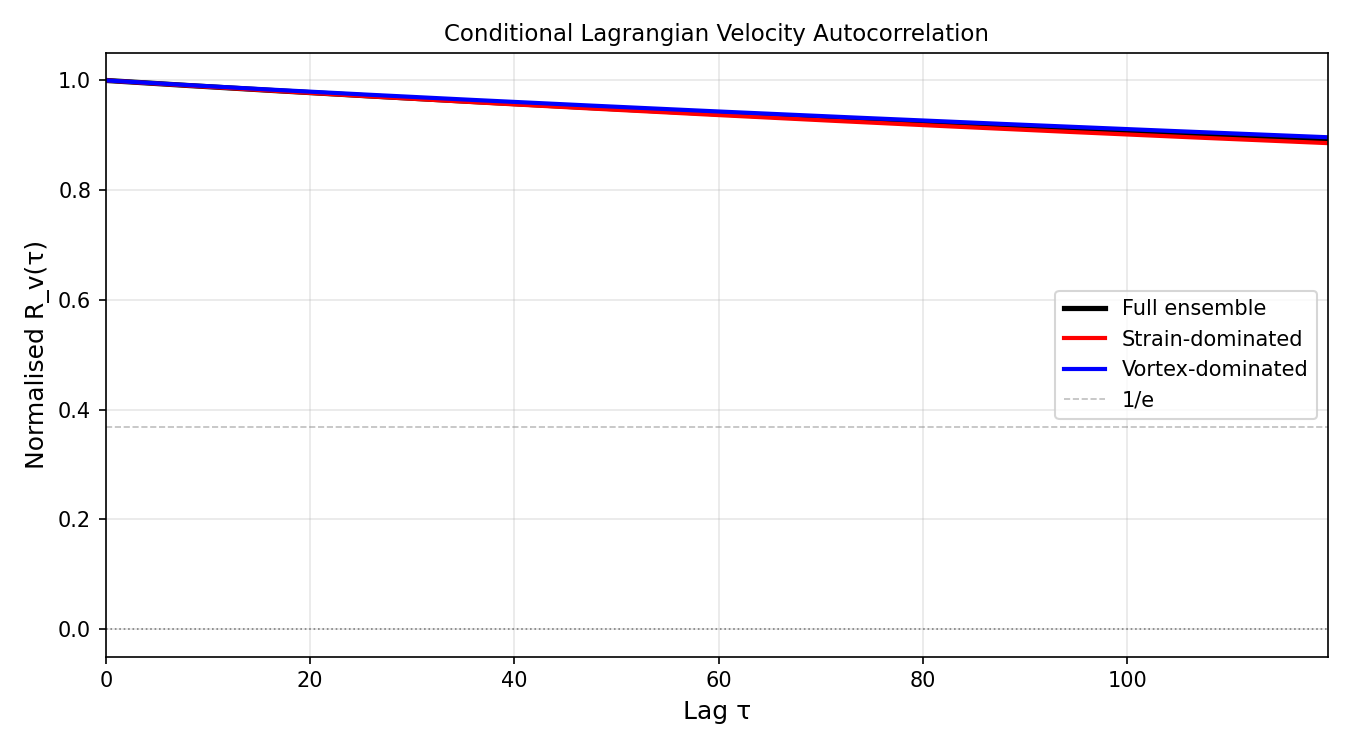
\includegraphics[width=0.99\textwidth]{../input_files/plots/iter2_conditional_Rv_1779134732.png}
    \caption{Normalised Lagrangian velocity autocorrelation function, $R_v(\tau)$, for the full tracer ensemble (black), the strain-dominated subpopulation ($>70\%$ time in strain, red), and the vortex-dominated subpopulation ($<30\%$ time in strain, blue). The slow decay indicates a long velocity correlation time, which drives the initial quasi-ballistic transport. The curves for the strain-dominated and vortex-dominated populations are nearly identical, refuting the hypothesis of distinct transport mechanisms and showing that long-term velocity correlations are homogeneous throughout the flow.}
    \label{fig:autocorrelation}
\end{figure*}

\subsection{Absence of Lévy-type statistics}

Finally, we examined the data for statistical signatures of other known mechanisms of anomalous diffusion, namely Lévy flights and Continuous Time Random Walks (CTRW). Lévy flights are generated by velocity increments with heavy-tailed, infinite-variance probability distributions. Our analysis shows this is not the case. The tails of the Lagrangian velocity increment distributions, $\delta \mathbf{v}(\tau)$, are characterized by a tail exponent $\beta > 3$ for all measured lag times and for all tracer sub-populations, confirming that the increments have finite variance. For the full ensemble, the exponent increases with lag time from $\beta \approx 3.36$ at $\tau=10$ to $\beta \approx 4.84$ at $\tau=500$.

Similarly, we find no evidence for a CTRW process, which requires a power-law distribution of trapping times with an exponent $\mu < 2$. The distribution of trapping times for particles within vortex cores did not exhibit such a power-law tail. The absence of these statistical markers strengthens our conclusion that the transport in this system is not truly anomalous, but is best described as a correlated random walk undergoing a slow crossover to normal diffusion.

\section{Conclusions}
\label{sec:conclusions}
In this work, we investigated the physical origin of apparent superdiffusive transport in forced two-dimensional turbulence, aiming to distinguish between theories based on long-range correlations and those based on intermittent, ballistic flights along strain-dominated `highways'. To this end, we analyzed Lagrangian particle trajectories from a direct numerical simulation. We partitioned the flow using the Okubo-Weiss criterion to classify tracers based on their history in strain- or vortex-dominated regions and compared their transport statistics against a memoryless null model generated from phase-randomized surrogate data.

Our analysis reveals that the system does not exhibit true, asymptotic superdiffusion. Instead, we observe a pre-asymptotic crossover phenomenon where the time-dependent Hurst exponent decays from a near-ballistic regime at short times towards the normal diffusive limit ($H=0.5$) at late times. The apparent superdiffusion is a transient feature of this long relaxation process. We find no evidence to support the `highway' hypothesis. Tracers that spend the majority of their time in strain-dominated regions show long-time transport scaling that is statistically indistinguishable from that of tracers predominantly trapped in vortices. Both sub-populations relax towards normal diffusion, refuting the idea that a distinct, ballistically transported population drives the enhanced transport.

The dominant mechanism governing the transport dynamics is found to be strong, restorative temporal correlations in the Lagrangian velocity field. A comparison with phase-randomized surrogate trajectories, which exhibit near-ballistic transport, shows that the true particle displacement is significantly suppressed. This demonstrates that the flow's memory is anti-persistent, actively working against long-range dispersion. This restorative effect is a direct consequence of particle trapping within coherent vortices, which introduces strong negative velocity correlations. Furthermore, we found no statistical signatures of Lévy-type processes or Continuous Time Random Walks, reinforcing our main conclusion.

In conclusion, for the simulated regime of forced two-dimensional turbulence, the observed superdiffusion is a finite-time artifact of a slow crossover from ballistic to normal diffusive motion. This long crossover time is not caused by spatial intermittency or enhanced transport along specific structures, but is instead governed by the powerful restorative effect of vortex trapping, which suppresses particle displacement and introduces long-lived, anti-persistent temporal correlations into the Lagrangian velocity field.


\bibliography{bibliography}{}
\bibliographystyle{unsrt}

\end{document}
